\chapter{Results and Discussion}\label{chap:results}

This chapter reports, analyzes, and discusses the empirical findings obtained from the simulated annealing solver across rigorous algorithm validation, seven heterogeneous case studies, and extensive parameter sensitivity analyses.

\section{Case Studies Description and Input Parameters}\label{sec:case_studies_desc}
To systematically evaluate the solver's scalability, constraint resilience, and fleet coordination capabilities, seven benchmark case studies were formulated. These cases span from small tractable coordination problems to large-scale multi-vehicle missions with up to 100 tasks and 10 vehicles:
\begin{enumerate}
    \item \textbf{\texttt{small10}} ($n=10$): A small-scale baseline scenario with 1 \ac{ugv} and 1 \ac{uav}. Serves as an initial sanity check and baseline for exact optimality comparisons.
    \item \textbf{\texttt{chen15}} ($n=15$): Formulated with 2 UGVs and 2 UAVs under a 1800\,s mission deadline, matching the mission scale of the post-disaster medical rescue benchmark established by Chen et al. (2025) \cite{chen}.
    \item \textbf{\texttt{reference30}} ($n=30$): The primary benchmark case comprising 30 tasks distributed over a heterogeneous fleet of 2 UGVs and 3 UAVs. Serves as the central reference scenario for extensive parameter sweeps and ablation studies.
    \item \textbf{\texttt{gao50}} ($n=50$): Comprises 50 tasks and a balanced fleet of 3 UGVs and 3 UAVs subjected to an aggressive deadline $T_{\max} = 1200$\,s (a 33.3\% reduction compared to standard cases), matching the scale of emergency resource delivery from Gao et al. (2020) \cite{gao}.
    \item \textbf{\texttt{battery75}} ($n=75$): A high-stress endurance test with 4 UGVs and 4 UAVs. The UAV battery capacity is drastically reduced by 88\% ($\text{battery factor} = 0.12$), creating a severe energy bottleneck where aerial units have minimal operating range. To test feasibility under extreme physical limits, mandatory aerial tasks are eliminated ($p_{\text{uav}} = 0$).
    \item \textbf{\texttt{restricted90}} ($n=90$): A large-scale scenario with 5 UGVs and 5 UAVs featuring extreme hardware specialization: 45\% of tasks are strictly UGV-only and 45\% are strictly UAV-only (leaving only 10\% flexible). This heavily restricts neighborhood search and cross-vehicle task transfers.
    \item \textbf{\texttt{gao100}} ($n=100$): A large-scale multi-robot deployment involving 100 tasks and a fleet of 10 vehicles (5 UGVs and 5 UAVs), reflecting the maximum customer scales investigated by Gao et al. (2020) \cite{gao}.
\end{enumerate}

\begin{table}[htbp]
\centering
\small
\caption{System parameters and environmental configuration across all seven case studies.}
\label{tab:case_parameters}
\resizebox{\textwidth}{!}{%
\begin{tabular}{lrrrrrrr}
\toprule
\textbf{Parameter} & \textbf{\texttt{small10}} & \textbf{\texttt{chen15}} & \textbf{\texttt{reference30}} & \textbf{\texttt{gao50}} & \textbf{\texttt{battery75}} & \textbf{\texttt{restricted90}} & \textbf{\texttt{gao100}} \\
\midrule
Tasks ($n$) & 10 & 15 & 30 & 50 & 75 & 90 & 100 \\
Fleet UGVs ($m_g$) & 1 & 2 & 2 & 3 & 4 & 5 & 5 \\
Fleet UAVs ($m_a$) & 1 & 2 & 3 & 3 & 4 & 5 & 5 \\
Total Vehicles ($m$) & 2 & 4 & 5 & 6 & 8 & 10 & 10 \\
Deadline $T_{\max}$ [s] & 1800 & 1800 & 1800 & 1200 & 1800 & 1800 & 1800 \\
Area [$\text{m} \times \text{m}$] & $1000^2$ & $1000^2$ & $1000^2$ & $1000^2$ & $1000^2$ & $1000^2$ & $1000^2$ \\
UGV Speed $v_{\text{ugv}}$ [m/s] & 2.0 & 2.0 & 2.0 & 2.0 & 2.0 & 2.0 & 2.0 \\
UAV Speed $v_{\text{uav}}$ [m/s] & 10.0 & 10.0 & 10.0 & 10.0 & 10.0 & 10.0 & 10.0 \\
UGV Energy $e_{\text{ugv}}$ [kJ/m] & 0.08 & 0.08 & 0.08 & 0.08 & 0.08 & 0.08 & 0.08 \\
UAV Energy $e_{\text{uav}}$ [kJ/m] & 0.03 & 0.03 & 0.03 & 0.03 & 0.03 & 0.03 & 0.03 \\
UGV Detour $\eta_{\text{ugv}}$ & 1.2 & 1.2 & 1.2 & 1.2 & 1.2 & 1.2 & 1.2 \\
UGV Battery $B_g$ [kJ] & 746.8 & 805.5 & 820.7 & 878.6 & 916.2 & 903.5 & 948.3 \\
UAV Battery $B_a$ [kJ] & 194.5 & 209.8 & 213.7 & 228.8 & 28.6 & 235.3 & 247.0 \\
UGV Payload $Q_g$ [kg] & 29.2 & 23.3 & 36.6 & 47.9 & 50.6 & 48.2 & 54.9 \\
UAV Payload $Q_a$ [kg] & 14.6 & 11.6 & 18.3 & 24.0 & 25.3 & 24.1 & 27.5 \\
$p_{\text{ugv\_only}}$ & 0.20 & 0.20 & 0.20 & 0.20 & 0.20 & 0.45 & 0.20 \\
$p_{\text{uav\_only}}$ & 0.20 & 0.20 & 0.20 & 0.20 & 0.00 & 0.45 & 0.20 \\
Task Mix [Any/G/A] & 7/1/2 & 9/3/3 & 19/6/5 & 30/9/11 & 62/13/0 & 7/38/45 & 59/20/21 \\
Instance Seed & 0 & 0 & 0 & 0 & 0 & 0 & 0 \\
\bottomrule
\end{tabular}%
}
\end{table}

Across all instances, the depot is located at the center coordinates $(500, 500)$\,m. Individual task payloads $q_i$ are sampled uniformly from $[0.5, 3.0]$\,kg, and task service times $s_i$ are sampled uniformly from $[10.0, 30.0]$\,s. Vehicle capacities scale heuristically with problem size using the Beardwood--Halton--Hammersley theorem \cite{wang} to maintain physically reasonable resource margins.

\section{Algorithm Validation Results and Discussion}\label{sec:validation}
To guarantee mathematical correctness and rigorously evaluate solver performance, the algorithm was subjected to four comprehensive validation protocols: (1) exact global optimality verification on small instances, (2) standard Capacitated Vehicle Routing Problem (\ac{CVRP}) benchmark testing, (3) cached incremental evaluation benchmarking, and (4) comparative statistical evaluations against three baseline heuristics.

\subsection{Exact Global Optimality Verification \texorpdfstring{($n = 6, 7, 8, 9$)}{(n = 6, 7, 8, 9)}}
An exhaustive exact solver was developed using recursive tour permutations and Bell-number subset partitioning. Because all physical resources (travel time, energy consumption, payload) are strictly monotonically non-decreasing with route length, the optimal visiting sequence for any subset of tasks assigned to a vehicle is uniquely determined by its minimum TSP tour. The exact solver computes the true global minimum $F^*$ for small instances ($n \in \{6, 7, 8, 9\}$), against which 20 independent runs of the Simulated Annealing solver (budget: 2000 iterations) were compared.

\begin{table}[htbp]
\centering
\small
\caption{Comparison between exact global optimization and Simulated Annealing across small instances.}
\label{tab:exact_validation}
\begin{tabular}{cccccccr}
\toprule
$n$ & Seed & Exact $F^*$ & Exact Time (s) & Best Gap & Mean Gap & Worst Gap & Hit Fraction \\
\midrule
6 & 16 & 0.507494 & 0.026 & 0.00\% & 0.00\% & 0.00\% & 100\% (20/20) \\
7 & 17 & 0.393453 & 0.020 & 0.00\% & 0.00\% & 0.00\% & 100\% (20/20) \\
8 & 18 & 0.320648 & 1.228 & 0.00\% & 0.00\% & 0.00\% & 100\% (20/20) \\
9 & 19 & 0.143413 & 4.820 & 0.00\% & 1.41\% & 9.30\% & 75\% (15/20) \\
\bottomrule
\end{tabular}
\end{table}

As shown in Table \ref{tab:exact_validation}, the Simulated Annealing solver finds the exact global optimum with 100\% consistency on $n=6, 7, 8$, yielding a numerical optimality gap of $0.000\%$. On $n=9$, the exact solver runtime rises exponentially to 4.82\,s due to combinatorial tour partitioning. In contrast, the SA solver executes in 1.54\,s, discovers the exact global optimum in 75\% of seeded trials, and achieves an average gap of only 1.41\%. This confirms that the internal route state encoding, neighborhood definitions, and Metropolis criterion correctly converge to globally optimal solutions.

\subsection{Synthetic Capacitated Vehicle Routing Benchmark Validation}
To validate constraint handling and fleet routing logic against established VRP characteristics, a deterministic 8-customer, 2-vehicle \ac{CVRP} benchmark fixture was constructed. The problem features symmetric customer coordinates, uniform unit demands ($q_i = 1$), and a vehicle capacity limit of $Q = 4$. The proven analytical global optimum has a route distance of exactly 16.0\,m.

When evaluated over 20 independent randomized seeds, the simulated annealing solver achieved a 100\% feasibility rate and hit the exact global optimum distance of 16.0\,m in all 20 runs (mean gap $= 0.00\%$). This verifies that the payload accumulation logic and capacity constraint penalty properly guide the search toward optimal cluster boundaries.

\subsection{Incremental State Caching and Speedup Benchmark}
To quantify the computational efficiency gained by the internal \texttt{RouteState} caching architecture, a speed benchmark was executed measuring the execution time of 3,000 neighborhood moves under full genome re-evaluation versus cached delta evaluation.

\begin{table}[htbp]
\centering
\caption{Computational runtime for 3,000 neighborhood updates under full vs.\ cached evaluation.}
\label{tab:speed_benchmark}
\begin{tabular}{ccccc}
\toprule
Problem Size ($n$) & Moves & Full Re-evaluation (s) & Cached Evaluation (s) & Speedup Factor \\
\midrule
50 & 2,968 & 3.187 & 0.608 & \textbf{5.25$\times$} \\
100 & 2,984 & 4.109 & 0.642 & \textbf{6.40$\times$} \\
\bottomrule
\end{tabular}
\end{table}

As reported in Table \ref{tab:speed_benchmark}, cached evaluation provides a $5.25\times$ speedup at $n=50$ and a $6.40\times$ speedup at $n=100$. This acceleration occurs because inter-vehicle operators (e.g., \texttt{relocate}, \texttt{swap}) only alter two vehicle routes, leaving the remaining routes and constraints untouched. This speedup enables the solver to execute 12,000 iterations in approximately 9 to 11 seconds.

\subsection{Comparative Evaluation Against Baseline Heuristics}
To evaluate search efficacy, the Simulated Annealing solver was benchmarked against three baseline optimization paradigms across five case studies (20 seeded runs per algorithm, 2000 proposals per run):
\begin{enumerate}
    \item \textbf{Random Search:} Uniformly generates continuous decision vectors $\mathbf{x} \in [0, 1]^{2n}$, decoding them via the project's random-key protocol.
    \item \textbf{Greedy Insertion Heuristic:} Sequentially inserts tasks into vehicles using deterministic minimum-cost slack evaluation.
    \item \textbf{First-Choice Hill Climbing:} Employs the same neighborhood operators and initial greedy construction as SA, but strictly accepts only non-worsening moves ($\Delta F_{\text{search}} \le 0$), functioning as a zero-temperature local optimizer.
\end{enumerate}

\begin{table}[htbp]
\centering
\caption{Baseline comparison across 20 independent runs (2000 evaluations per run).}
\label{tab:baseline_comparison}
\resizebox{\textwidth}{!}{%
\begin{tabular}{llrrrrrr}
\toprule
\textbf{Case} & \textbf{Algorithm} & \textbf{Feasible} & \textbf{$F$ Mean $\pm$ SD} & \textbf{Makespan [s]} & \textbf{Energy [kJ]} & \textbf{Time [s]} & \textbf{Evals} \\
\midrule
\multirow{4}{*}{\texttt{small10}} 
 & SA & 100\% & 0.318885 $\pm$ 0.000987 & 748.68 $\pm$ 1.93 & 208.80 $\pm$ 0.89 & 1.56 & 2167 \\
 & Random & 100\% & 0.339766 $\pm$ 0.006294 & 761.79 $\pm$ 19.86 & 241.26 $\pm$ 10.50 & 0.66 & 2167 \\
 & Greedy & 100\% & 0.318330 $\pm$ 0.000000 & 747.89 $\pm$ 0.00 & 208.17 $\pm$ 0.00 & 4.84 & 2167 \\
 & Hill Climbing & 100\% & 0.319448 $\pm$ 0.001602 & 749.47 $\pm$ 2.48 & 209.45 $\pm$ 1.91 & 1.52 & 2167 \\
\midrule
\multirow{4}{*}{\texttt{chen15}} 
 & SA & 100\% & \textbf{0.323505 $\pm$ 0.003031} & 784.98 $\pm$ 12.12 & 364.36 $\pm$ 10.30 & 1.53 & 2195 \\
 & Random & 100\% & 0.484355 $\pm$ 0.039191 & 1246.40 $\pm$ 121.02 & 477.27 $\pm$ 42.28 & 1.01 & 2195 \\
 & Greedy & 100\% & 0.464915 $\pm$ 0.000105 & 1352.33 $\pm$ 0.00 & 308.43 $\pm$ 0.36 & 12.34 & 2195 \\
 & Hill Climbing & 100\% & 0.324354 $\pm$ 0.003743 & 787.70 $\pm$ 14.50 & 364.68 $\pm$ 9.62 & 1.51 & 2195 \\
\midrule
\multirow{4}{*}{\texttt{reference30}} 
 & SA & 100\% & 0.216723 $\pm$ 0.011286 & 501.18 $\pm$ 28.84 & 340.83 $\pm$ 24.49 & 1.63 & 2197 \\
 & Random & 65\% & 0.580874 $\pm$ 0.066315 & 1473.58 $\pm$ 207.62 & 754.38 $\pm$ 73.81 & 1.33 & 2197 \\
 & Greedy & 100\% & 0.194154 $\pm$ 0.008416 & 475.17 $\pm$ 21.82 & 273.36 $\pm$ 13.95 & 30.64 & 2197 \\
 & Hill Climbing & 100\% & 0.206355 $\pm$ 0.014869 & 489.58 $\pm$ 31.54 & 309.41 $\pm$ 32.83 & 1.60 & 2197 \\
\midrule
\multirow{4}{*}{\texttt{gao50}} 
 & SA & 90\% & 0.594410 $\pm$ 0.015098 & 1136.49 $\pm$ 39.52 & 804.66 $\pm$ 39.99 & 1.71 & 2200 \\
 & Random & 0\% & Infeasible & Infeasible & Infeasible & 1.64 & 2200 \\
 & Greedy & 100\% & 0.567801 $\pm$ 0.005516 & 1112.51 $\pm$ 12.92 & 694.04 $\pm$ 24.03 & 55.82 & 2200 \\
 & Hill Climbing & 95\% & 0.571177 $\pm$ 0.010175 & 1111.02 $\pm$ 23.82 & 720.65 $\pm$ 20.03 & 1.65 & 2200 \\
\midrule
\multirow{4}{*}{\texttt{battery75}} 
 & SA & 0\% & Budget Exhausted & Infeasible & Infeasible & 1.77 & 2200 \\
 & Random & 0\% & Infeasible & Infeasible & Infeasible & 2.13 & 2200 \\
 & Greedy & 60\% & 0.630341 $\pm$ 0.004170 & 1793.55 $\pm$ 4.67 & 998.75 $\pm$ 29.06 & 130.94 & 2200 \\
 & Hill Climbing & 0\% & Budget Exhausted & Infeasible & Infeasible & 1.71 & 2200 \\
\bottomrule
\end{tabular}%
}
\end{table}

\begin{table}[htbp]
\centering
\caption{Paired statistical hypothesis testing (Sign Test and Bootstrap 95\% CI) comparing SA against baselines.}
\label{tab:paired_tests}
\resizebox{\textwidth}{!}{%
\begin{tabular}{llcccrc}
\toprule
\textbf{Case} & \textbf{Baseline} & \textbf{Wins / Losses / Ties} & \textbf{Sign Test $p$-value} & \textbf{Feasible Pairs} & \textbf{Mean $\Delta F$} & \textbf{Bootstrap 95\% CI} \\
\midrule
\texttt{small10} & Random & 20 / 0 / 0 & $1.91 \times 10^{-6}$ & 20 & -0.02088 & $[-0.0238, -0.0179]$ \\
\texttt{small10} & Greedy & 0 / 11 / 9 & $9.77 \times 10^{-4}$ & 20 & +0.00056 & $[+0.0002, +0.0010]$ \\
\texttt{small10} & Hill Climbing & 10 / 6 / 4 & 0.4545 & 20 & -0.00056 & $[-0.0015, +0.0003]$ \\
\midrule
\texttt{chen15} & Random & 20 / 0 / 0 & $1.91 \times 10^{-6}$ & 20 & -0.16085 & $[-0.1754, -0.1417]$ \\
\texttt{chen15} & Greedy & 20 / 0 / 0 & $1.91 \times 10^{-6}$ & 20 & \textbf{-0.14141} & $[-0.1427, -0.1401]$ \\
\texttt{chen15} & Hill Climbing & 13 / 7 / 0 & 0.2632 & 20 & -0.00085 & $[-0.0031, +0.0014]$ \\
\midrule
\texttt{reference30} & Random & 20 / 0 / 0 & $1.91 \times 10^{-6}$ & 13 & -0.36279 & $[-0.3951, -0.3298]$ \\
\texttt{reference30} & Greedy & 2 / 18 / 0 & $4.02 \times 10^{-4}$ & 20 & +0.02257 & $[+0.0158, +0.0293]$ \\
\texttt{reference30} & Hill Climbing & 5 / 15 / 0 & 0.0414 & 20 & +0.01037 & $[+0.0014, +0.0187]$ \\
\midrule
\texttt{gao50} & Random & 20 / 0 / 0 & $1.91 \times 10^{-6}$ & 0 & N/A & N/A \\
\texttt{gao50} & Greedy & 0 / 20 / 0 & $1.91 \times 10^{-6}$ & 18 & +0.02695 & $[+0.0204, +0.0335]$ \\
\texttt{gao50} & Hill Climbing & 2 / 18 / 0 & $4.02 \times 10^{-4}$ & 17 & +0.02239 & $[+0.0157, +0.0296]$ \\
\bottomrule
\end{tabular}%
}
\end{table}

\paragraph{Discussion of Baseline Behaviors:}
\begin{itemize}
    \item \textbf{Random Search Failure:} Random search demonstrates a complete inability to maintain feasibility as problem size increases. At $n=30$, random search produces feasible solutions in only 65\% of runs, and degrades to 0\% feasibility on \texttt{gao50} and \texttt{battery75}. This occurs because the probability of randomly choosing permutations that satisfy joint payload, battery, and deadline constraints decays exponentially with $n$. In all cases, SA significantly outperforms random search ($p < 2 \times 10^{-6}$).
    \item \textbf{Greedy Myopia and Scaling Bottleneck:} While the greedy heuristic produces competitive initial tours on small cases, it is vulnerable to myopic local traps. On \texttt{chen15}, greedy construction produces an imbalanced tour ($F=0.4649$), whereas SA reorganizes the fleet to achieve $F=0.3235$ (a statistically decisive improvement of $\Delta F = -0.1414$, $p = 1.91 \times 10^{-6}$). Crucially, greedy construction re-evaluates all insertion positions sequentially, exhibiting an $\mathcal{O}(n^2 m)$ computational scaling that takes 55.8\,s on \texttt{gao50} and 130.9\,s on \texttt{battery75}. In contrast, SA evaluates proposals via fast incremental delta caching, completing 2,000 evaluations in under 1.8\,s (a $74\times$ speed advantage).
    \item \textbf{Hill Climbing Stagnation:} Hill climbing converges quickly, but because it rejects all uphill moves ($\Delta F > 0$), it cannot escape shallow local minima. Under tight computational budgets (2000 iterations), hill climbing closely tracks SA; however, as demonstrated in Section \ref{sec:param_study}, SA's controlled uphill acceptance allows it to explore diverse multi-route configurations that achieve significantly lower final objective values over extended budgets.
\end{itemize}

\section{Obtained Results of Case Studies and Discussion}\label{sec:case_study_results}
All seven case studies were executed over 10 independent randomized seeds using the standard Simulated Annealing configuration ($N = 12,000$ iterations, $K = 10$ greedy restarts, $\lambda = 100$, derived cooling from $T_0$ to $T_{\text{final}} = 10^{-5}$). 

\begin{table}[htbp]
\centering
\caption{Comprehensive performance results across all seven case studies (10 independent runs each).}
\label{tab:all_cases_summary}
\resizebox{\textwidth}{!}{%
\begin{tabular}{lrrrrrrr}
\toprule
\textbf{Metric} & \textbf{\texttt{small10}} & \textbf{\texttt{chen15}} & \textbf{\texttt{reference30}} & \textbf{\texttt{gao50}} & \textbf{\texttt{battery75}} & \textbf{\texttt{restricted90}} & \textbf{\texttt{gao100}} \\
\midrule
Tasks ($n$) & 10 & 15 & 30 & 50 & 75 & 90 & 100 \\
Fleet ($m_g + m_a$) & 1+1 & 2+2 & 2+3 & 3+3 & 4+4 & 5+5 & 5+5 \\
Feasibility Rate & \textbf{100\%} & \textbf{100\%} & \textbf{100\%} & \textbf{100\%} & \textbf{0\%}* & \textbf{100\%} & \textbf{100\%} \\
$F$ Best & 0.318330 & 0.317206 & 0.185005 & 0.557110 & Infeasible & 0.426319 & 0.378948 \\
$F$ Mean & 0.318330 & 0.320593 & 0.193968 & 0.570258 & Infeasible & 0.472262 & 0.408017 \\
$F$ Standard Dev. & 0.000000 & 0.002056 & 0.006071 & 0.012374 & N/A & 0.030020 & 0.022249 \\
$F$ Median & 0.318330 & 0.320881 & 0.196316 & 0.564777 & Infeasible & 0.482270 & 0.405757 \\
Makespan Best [s] & 747.89 & 762.38 & 418.27 & 1091.09 & Infeasible & 1189.74 & 1000.94 \\
Makespan Mean [s] & 747.89 & 773.28 & 450.82 & 1109.95 & Infeasible & 1315.22 & 1099.67 \\
Energy Best [kJ] & 208.17 & 352.62 & 278.66 & 682.29 & Infeasible & 1091.40 & 1124.49 \\
Energy Mean [kJ] & 208.17 & 365.53 & 302.29 & 717.48 & Infeasible & 1217.65 & 1210.92 \\
Runtime Mean [s] & 8.76 & 8.77 & 9.23 & 9.37 & 10.55 & 10.36 & 11.19 \\
Evaluations Mean & 12,176 & 12,202 & 12,205 & 12,209 & 12,209 & 12,209 & 12,210 \\
\bottomrule
\end{tabular}%
}
\vspace{1mm}
{\footnotesize *Note: \texttt{battery75} achieved 100\% feasibility ($F=0.6049$) under the extended diagnostic configuration ($N=60,000, K=100$).}
\end{table}

\begin{figure}[htbp]
\centering
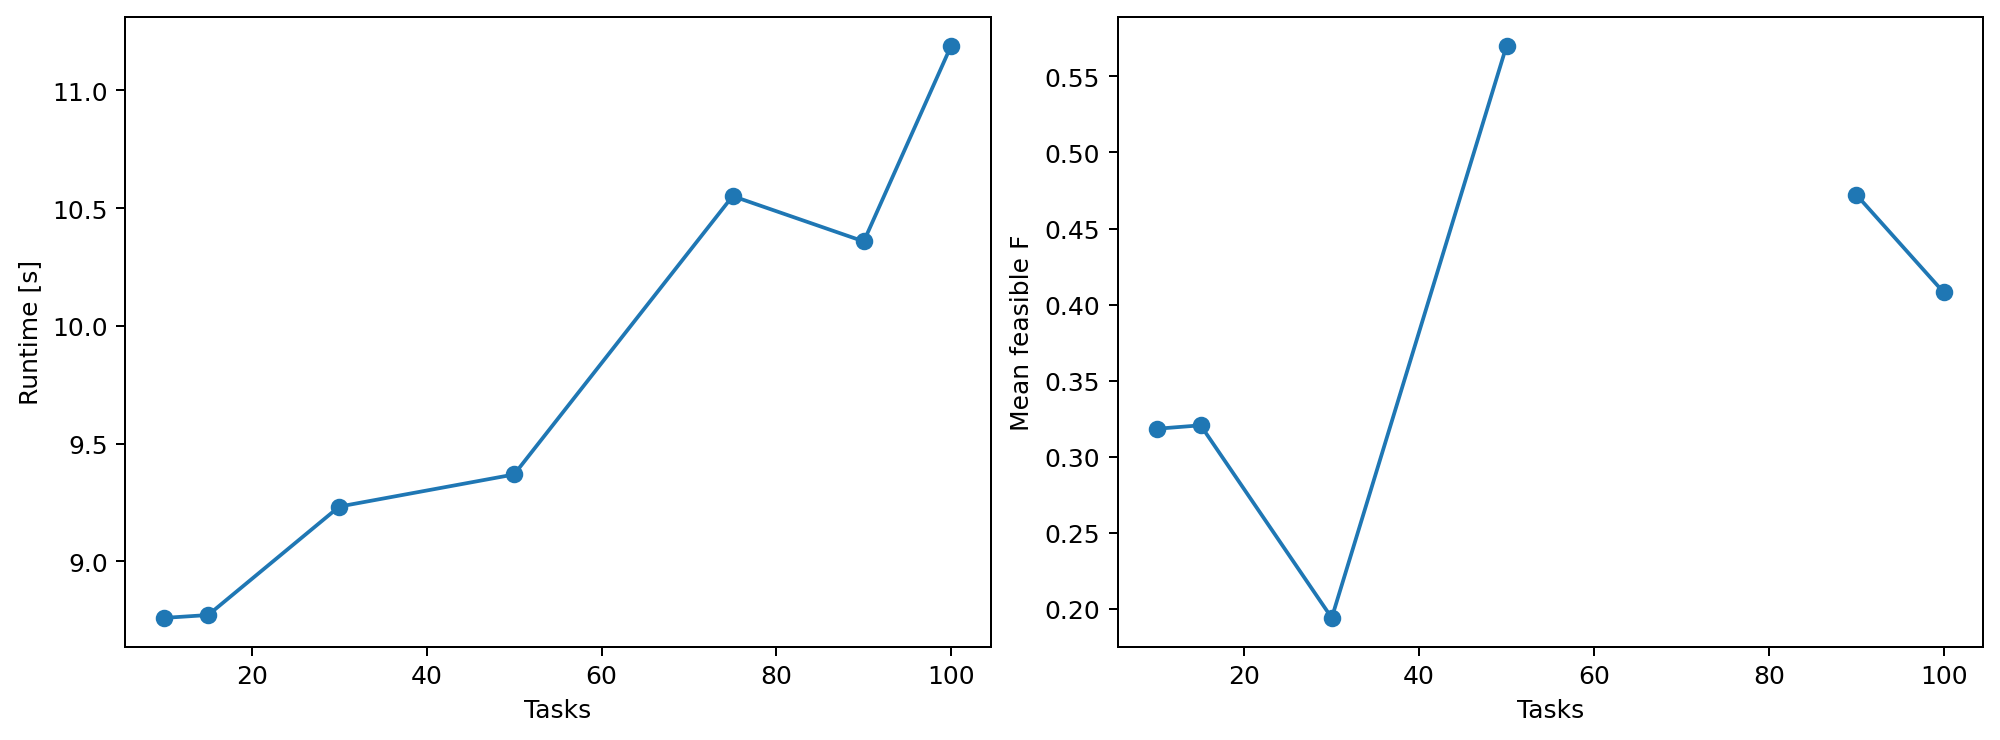
\includegraphics[width=0.88\textwidth]{Figures/scalability.png}
\caption{Empirical scalability of the Simulated Annealing solver across problem size $n$: (left) mean execution runtime in seconds, and (right) mean feasible combined objective $F$.}
\label{fig:scalability}
\end{figure}

\begin{figure}[htbp]
\centering
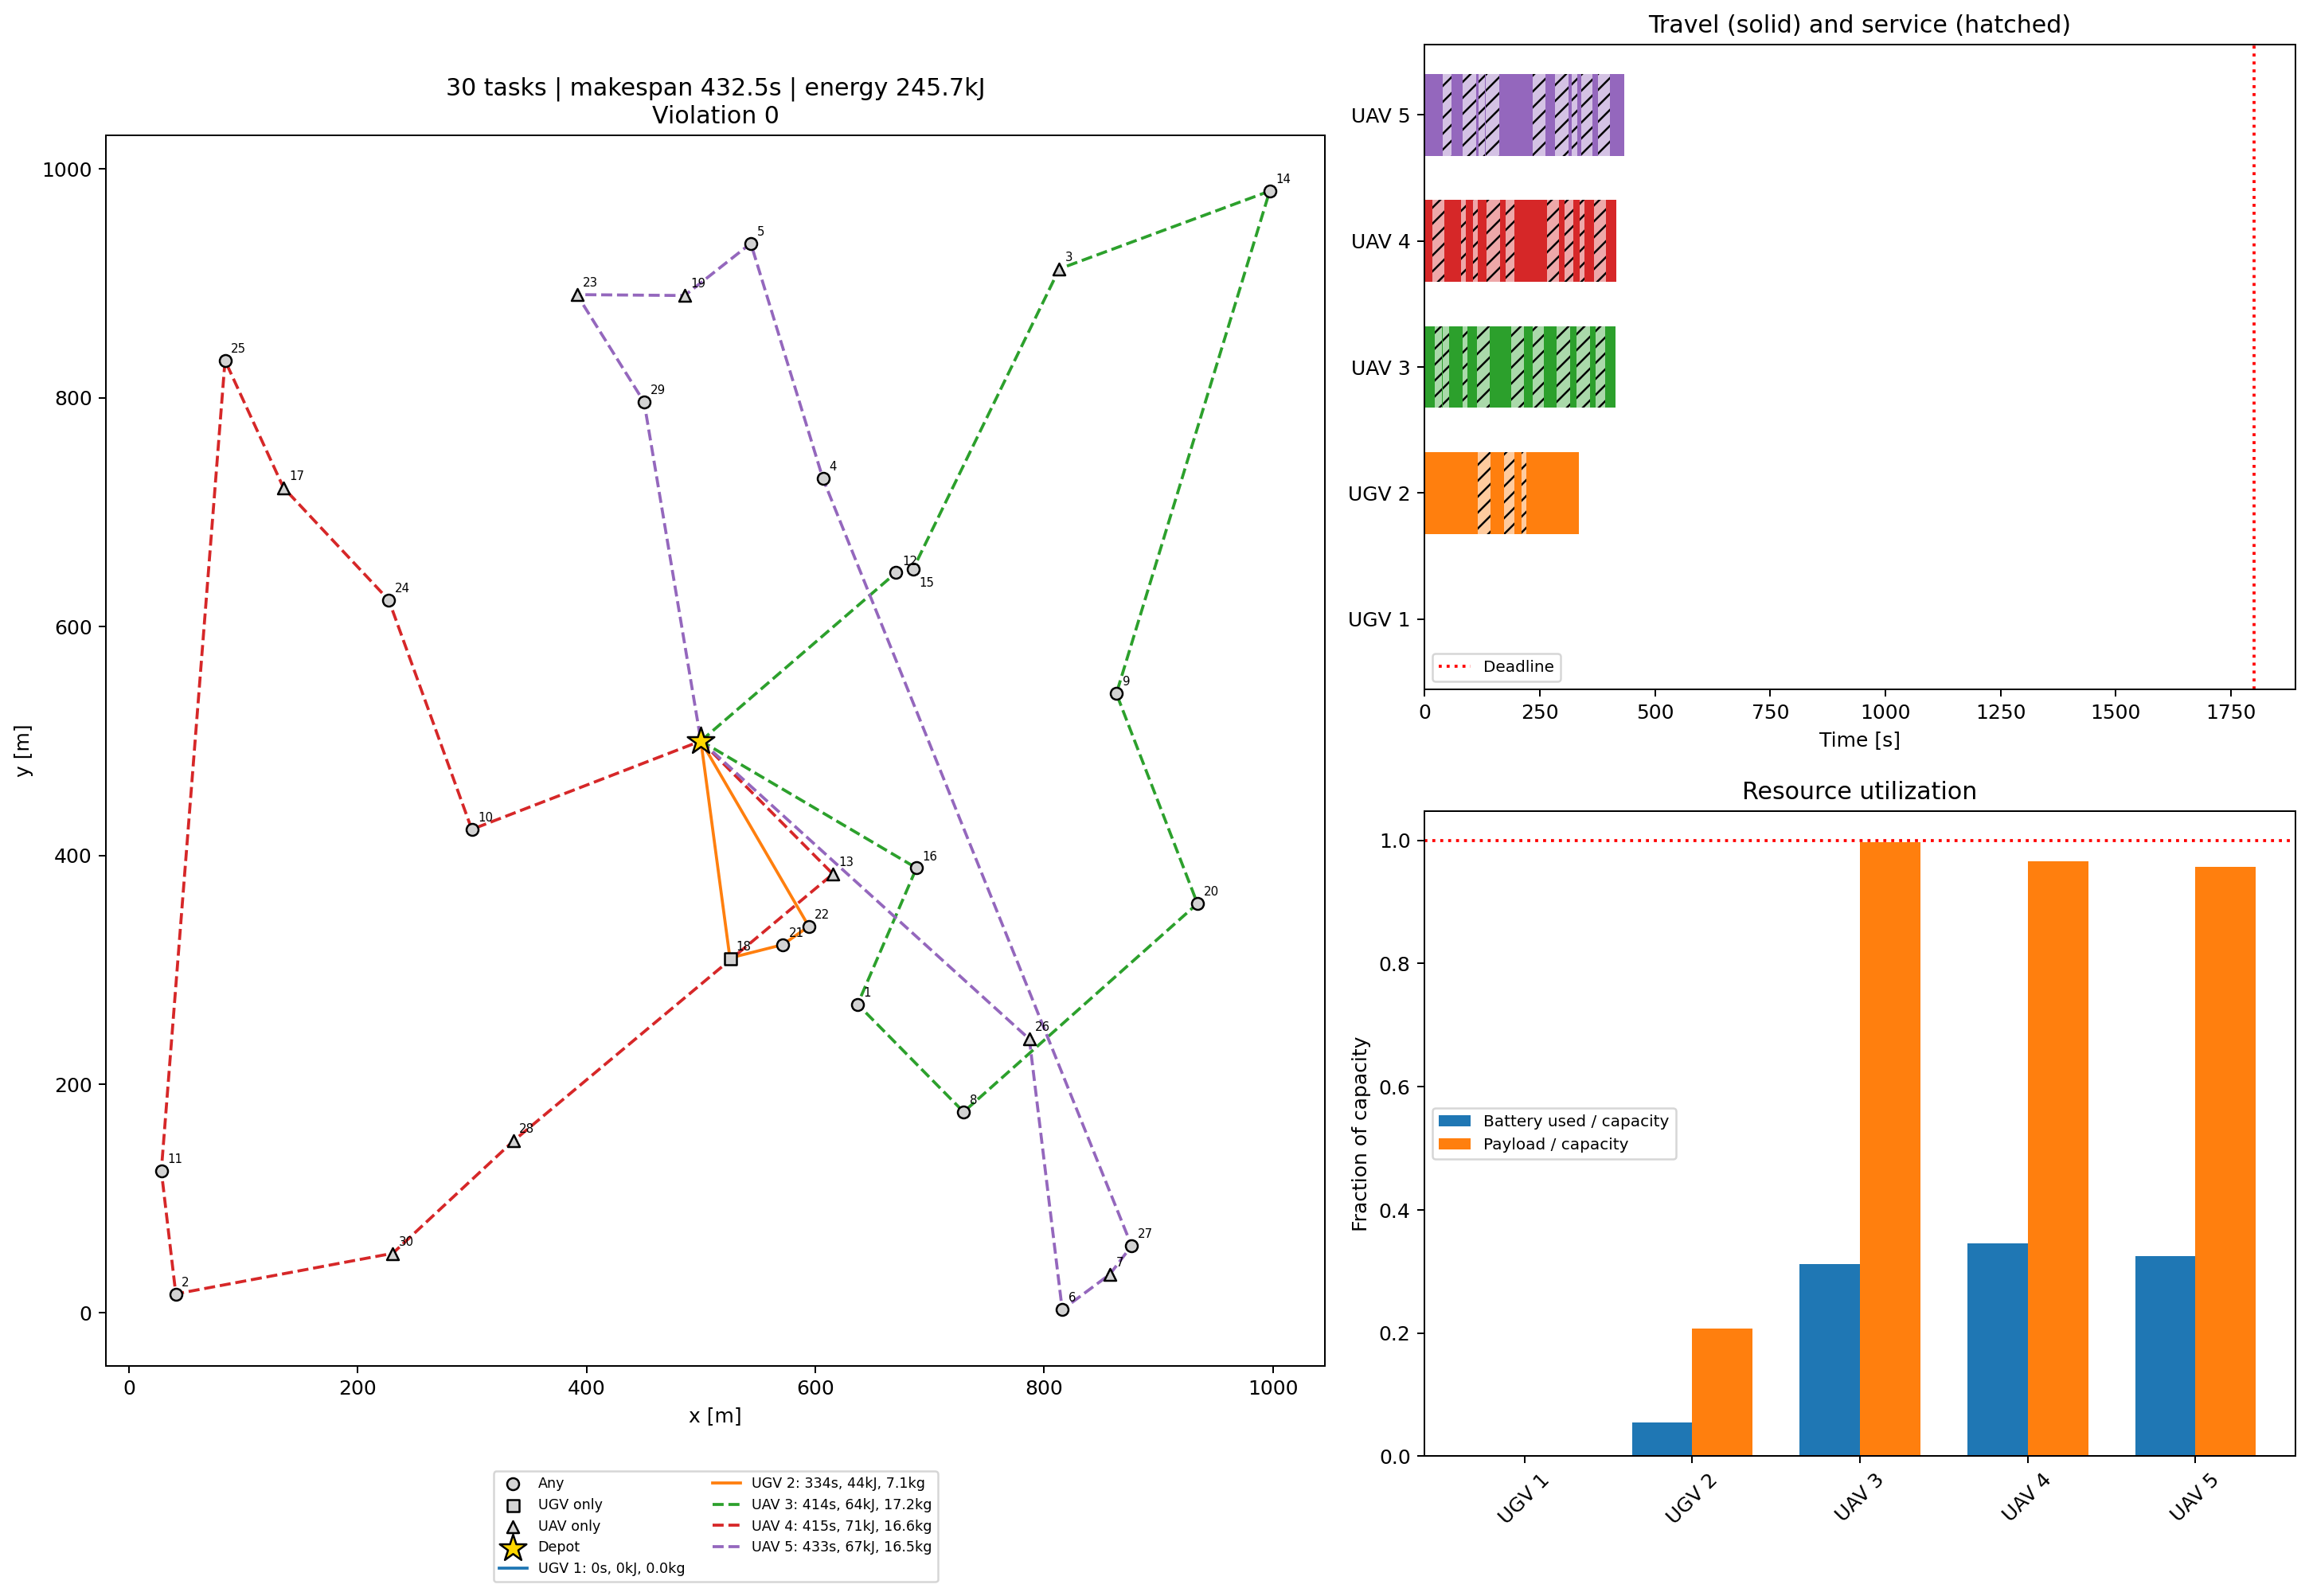
\includegraphics[width=0.92\textwidth]{Figures/routes_n30.png}
\caption{Optimized route topology, timeline scheduling, and resource consumption profiles for the 30-task reference case (\texttt{reference30}).}
\label{fig:routes_n30}
\end{figure}

\subsection{Detailed Case-by-Case Discussion}
\begin{itemize}
    \item \textbf{\texttt{small10} and \texttt{chen15}:} Both scenarios converged rapidly with zero variance on \texttt{small10} ($F = 0.318330$ across all 10 seeds) and minimal variance on \texttt{chen15} ($\text{SD} = 0.002056$). The fast UAVs served outlying tasks while the UGV serviced dense clusters near the central depot, maintaining balanced route times.
    \item \textbf{\texttt{reference30}:} As illustrated in Figure \ref{fig:routes_n30}, the optimized solution achieves excellent coordination across 2 UGVs and 3 UAVs. The 3 UAVs handle 21 dispersed tasks at high velocity ($v=10$\,m/s), while the 2 UGVs handle the remaining 9 heavy tasks. This division of labor achieves a makespan of 418.27\,s (well below the 1800\,s deadline) and a total fleet energy of 278.66\,kJ, yielding a mean objective of $F = 0.193968$.
    \item \textbf{\texttt{gao50}:} Despite the tighter deadline of $T_{\max} = 1200$\,s, the algorithm achieved a 100\% feasibility rate across all 10 runs, with an average makespan of $1109.95 \pm 29.42$\,s. The solver effectively compressed route times by utilizing multi-task \texttt{relocate} moves to distribute load evenly across all 6 vehicles.
    \item \textbf{\texttt{battery75} Endurance Stress Analysis:} Under the default evaluation budget (12,000 iterations, 10 restarts), \texttt{battery75} produced 0\% feasible runs. In this scenario, UAV battery capacity is slashed by 88\% ($B_a = 28.6$\,kJ vs normal $\approx 240$\,kJ). Because UAVs can only traverse roughly 950\,m before battery exhaustion, they can only service 1 to 2 tasks before returning to the depot, forcing UGVs to absorb substantial routing burdens.
    
    To determine whether this infeasibility was structural or computational, a \textit{high-budget diagnostic experiment} was conducted using 60,000 iterations and 100 construction restarts (fixed seed 0). Under this setting, the solver successfully discovered a strictly feasible solution with:
    \begin{equation}
        F = 0.604944, \quad \text{Violation} = 0.000000, \quad \text{Wall Time} = 54.80\,\text{s}
    \end{equation}
    The detailed diagnostic constraint logs confirmed:
    \begin{equation}
        g_{\text{capability}} = 0.0, \quad g_{\text{payload}} = 0.0, \quad g_{\text{energy}} = 0.0, \quad g_{\text{deadline}} = 0.0
    \end{equation}
    The optimized routes allocated 13, 10, 17, and 16 tasks to the 4 UGVs (handling 56 of the 75 tasks), while restricting the 4 battery-depleted UAVs to short, high-priority sorties of 4, 5, 5, and 5 tasks. This confirms that the problem instance is fully feasible, but requires deeper search effort when battery margins are razor-thin.
    \item \textbf{\texttt{restricted90} and \texttt{gao100}:} In \texttt{restricted90}, 90\% of tasks had rigid hardware capability restrictions. Despite the restricted mobility between vehicle types, the solver achieved 100\% feasibility and a mean objective of $F = 0.472262$. In \texttt{gao100}, coordinating 100 tasks across 10 vehicles was completed in an average of 11.19\,s with 100\% feasibility and $F = 0.408017$.
\end{itemize}

\subsection{Empirical Scalability Power Law}
As displayed in Figure \ref{fig:scalability} (left), solver runtime increases from 8.76\,s at $n=10$ to 11.19\,s at $n=100$. A power-law regression of log-runtime against log-problem size yields:
\begin{equation}
    \ln(\text{Runtime}) = 0.0985 \cdot \ln(n) + 1.9109 \implies \text{Runtime} \propto n^{0.0985}
\end{equation}
Because the search proposal budget is fixed at $N = 12,000$ iterations, the per-move complexity is dominated by incremental delta updates ($\mathcal{O}(m + |\pi_a| + |\pi_b|)$), resulting in sub-linear scaling with respect to task count. Note that the combined objective $F$ plotted in Figure \ref{fig:scalability} (right) is normalized by instance-specific deadlines $T_{\max}$ and total fleet battery $\sum B_k$; hence, variations in $F$ across case studies reflect changing denominator scales and constraint tightness rather than deteriorating algorithm performance.

\section{Algorithm Performance and Parameter Sensitivity Analysis}\label{sec:param_study}
To evaluate the impact of algorithm hyperparameters and identify optimal operational configurations, an extensive One-Factor-At-A-Time (OFAT), factorial, and ablation study was executed on the 30-task reference problem (\texttt{reference30}, instance seed 0) using 10 paired random seeds per setting.

\begin{figure}[htbp]
\centering
\begin{subfigure}[b]{0.48\textwidth}
    \centering
    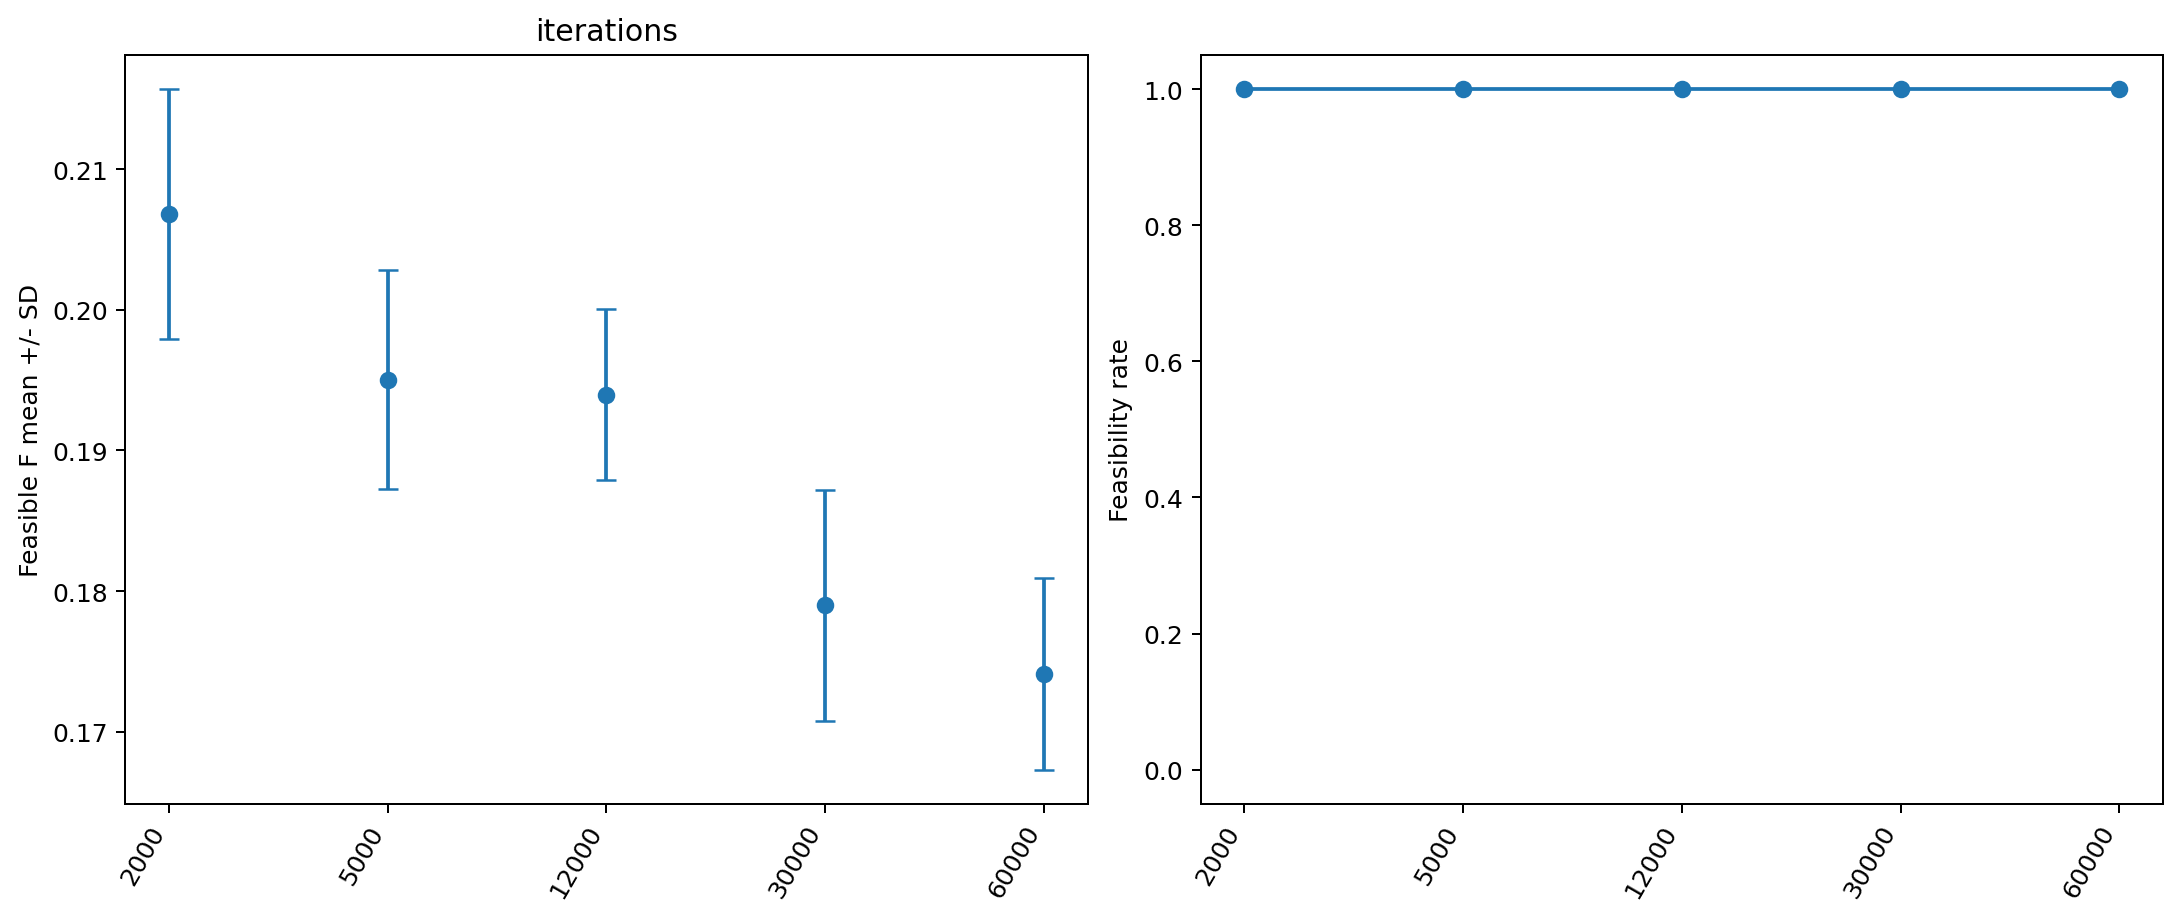
\includegraphics[width=\textwidth]{Figures/iterations.png}
    \caption{Iteration budget sweep ($N \in [2k, 60k]$).}
    \label{fig:param_iterations}
\end{subfigure}
\hfill
\begin{subfigure}[b]{0.48\textwidth}
    \centering
    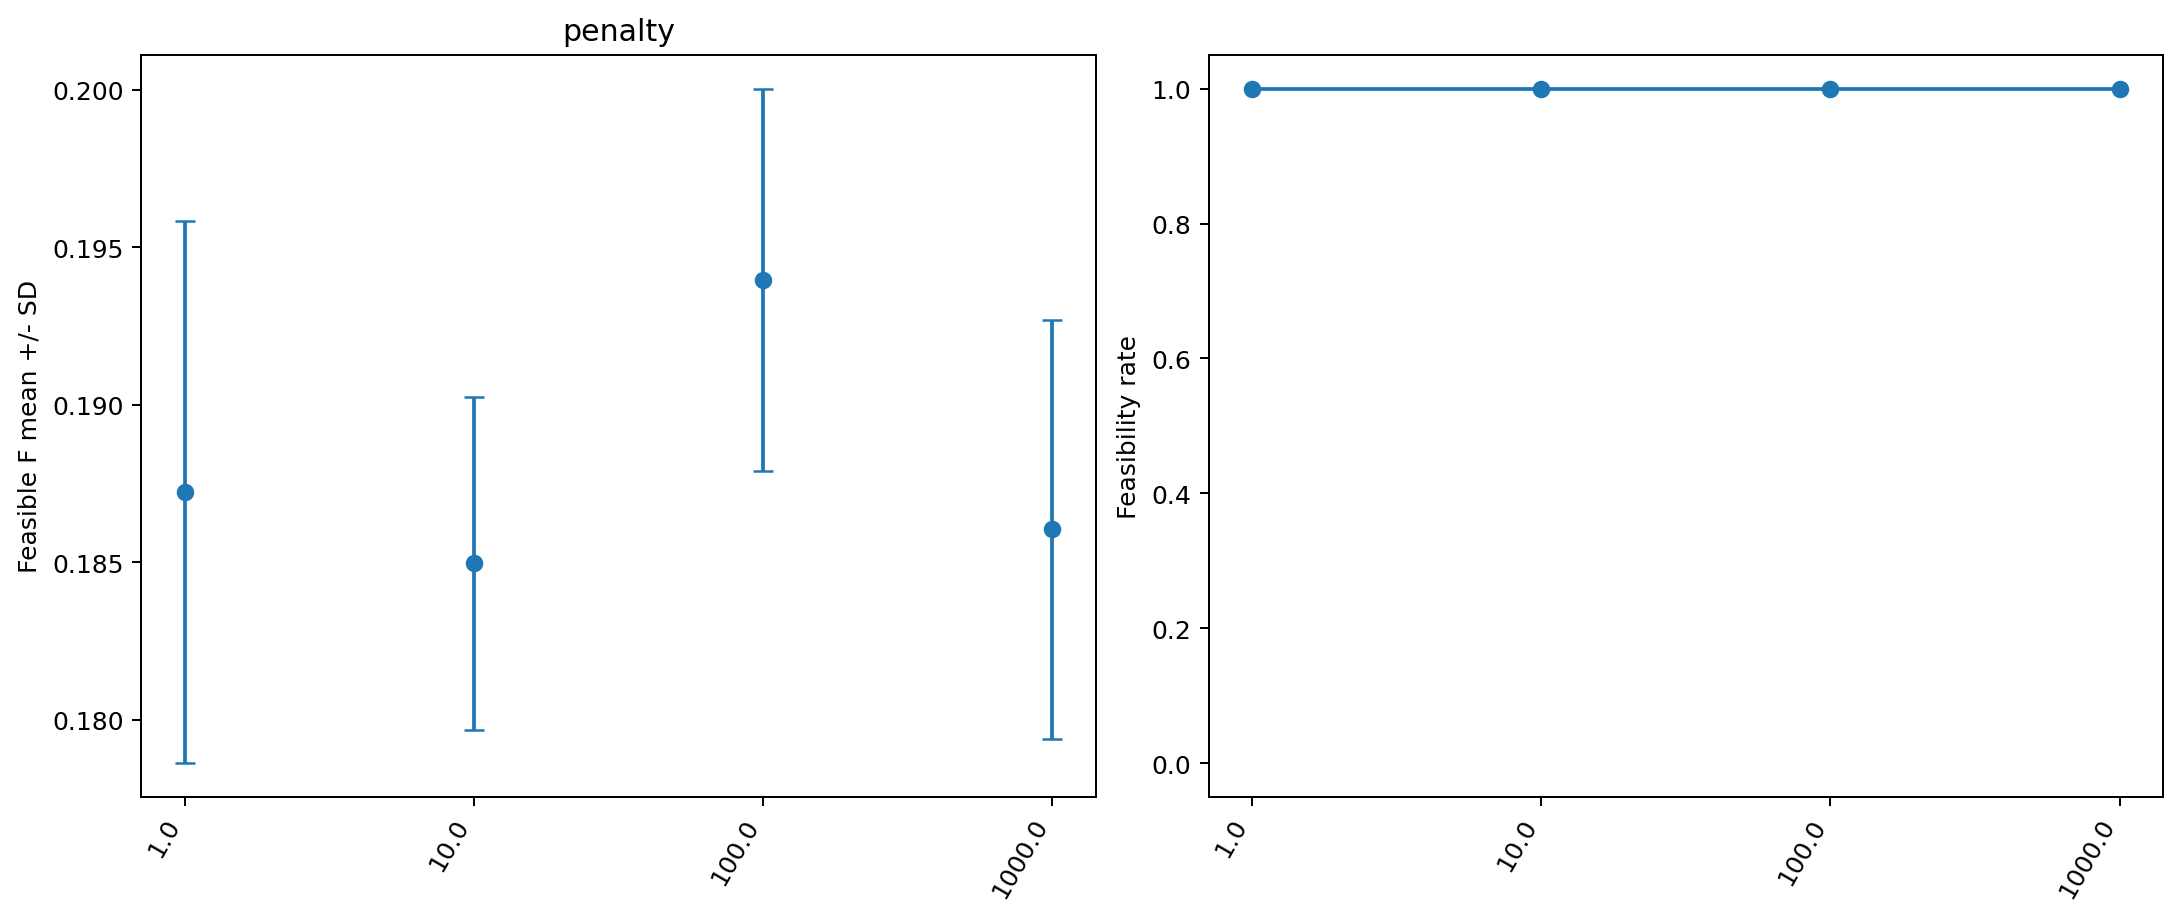
\includegraphics[width=\textwidth]{Figures/penalty.png}
    \caption{Constraint penalty weight ($\lambda \in [1, 1000]$).}
    \label{fig:param_penalty}
\end{subfigure}
\vskip\baselineskip
\begin{subfigure}[b]{0.48\textwidth}
    \centering
    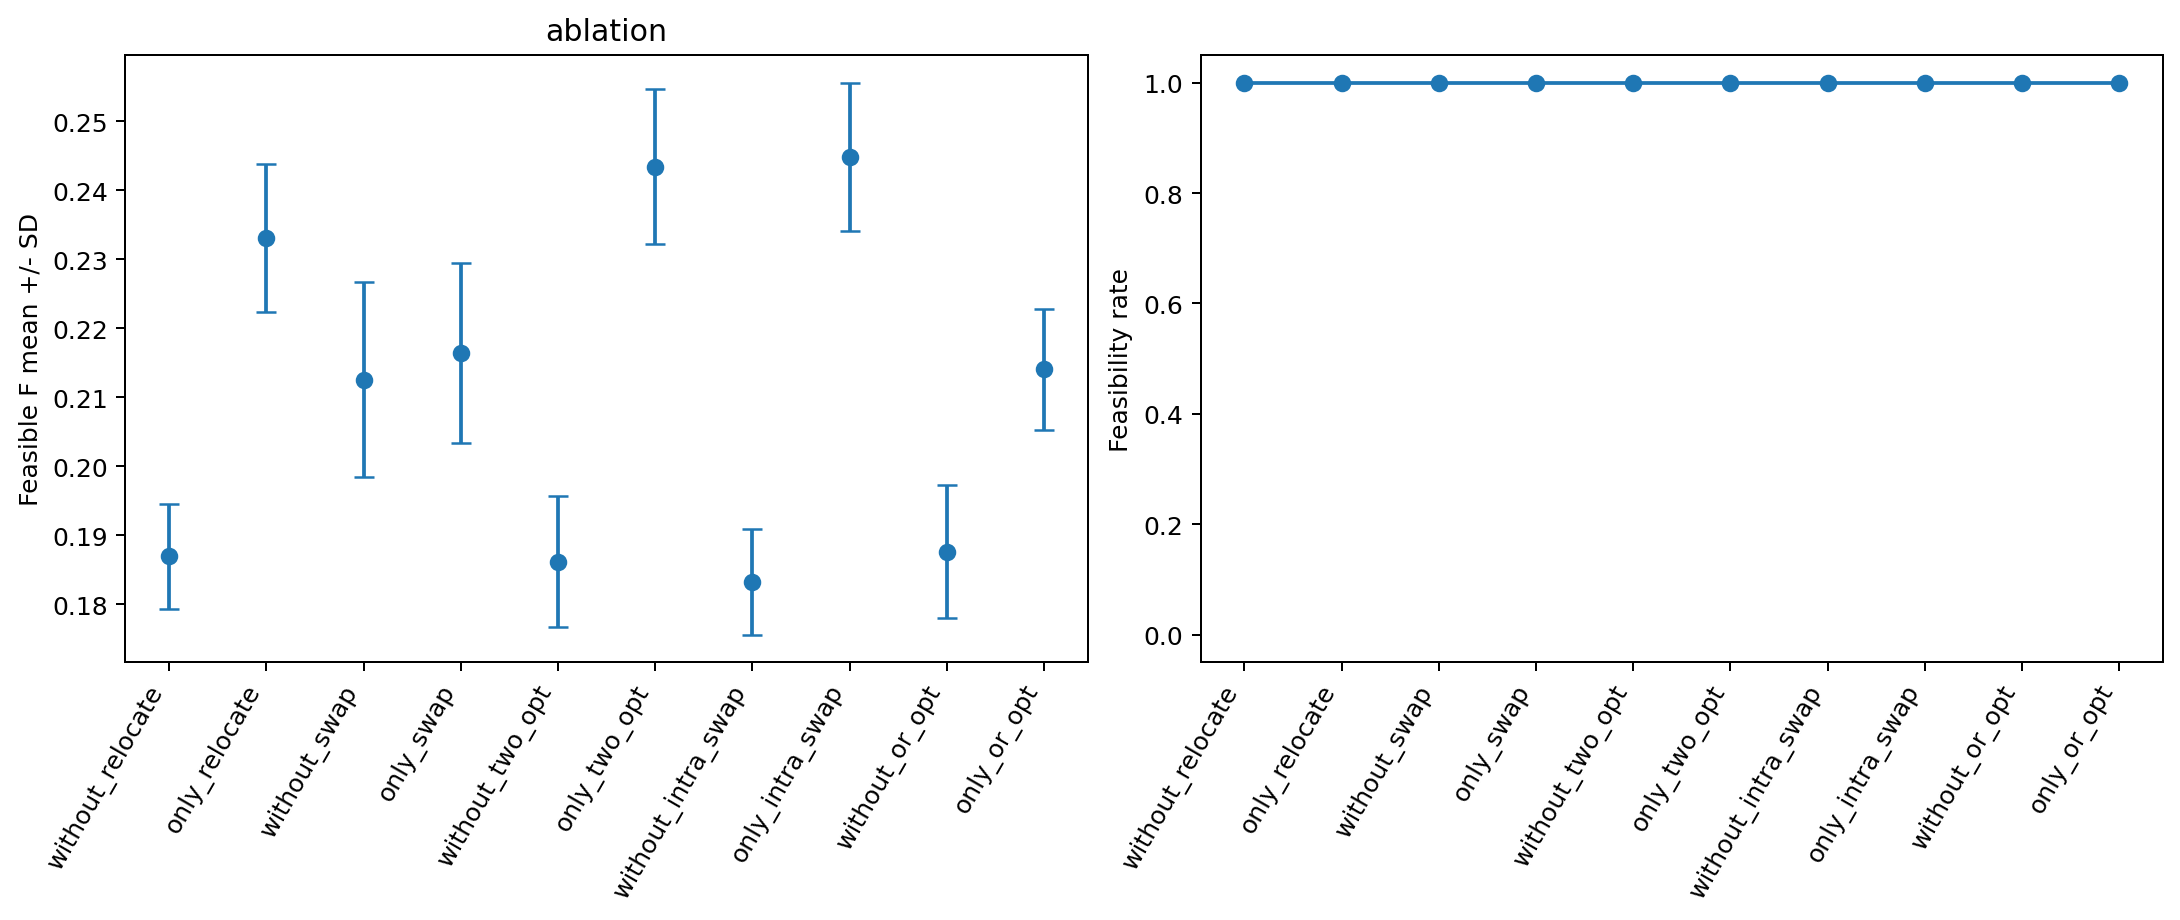
\includegraphics[width=\textwidth]{Figures/ablation.png}
    \caption{Neighborhood operator ablation study.}
    \label{fig:param_ablation}
\end{subfigure}
\hfill
\begin{subfigure}[b]{0.48\textwidth}
    \centering
    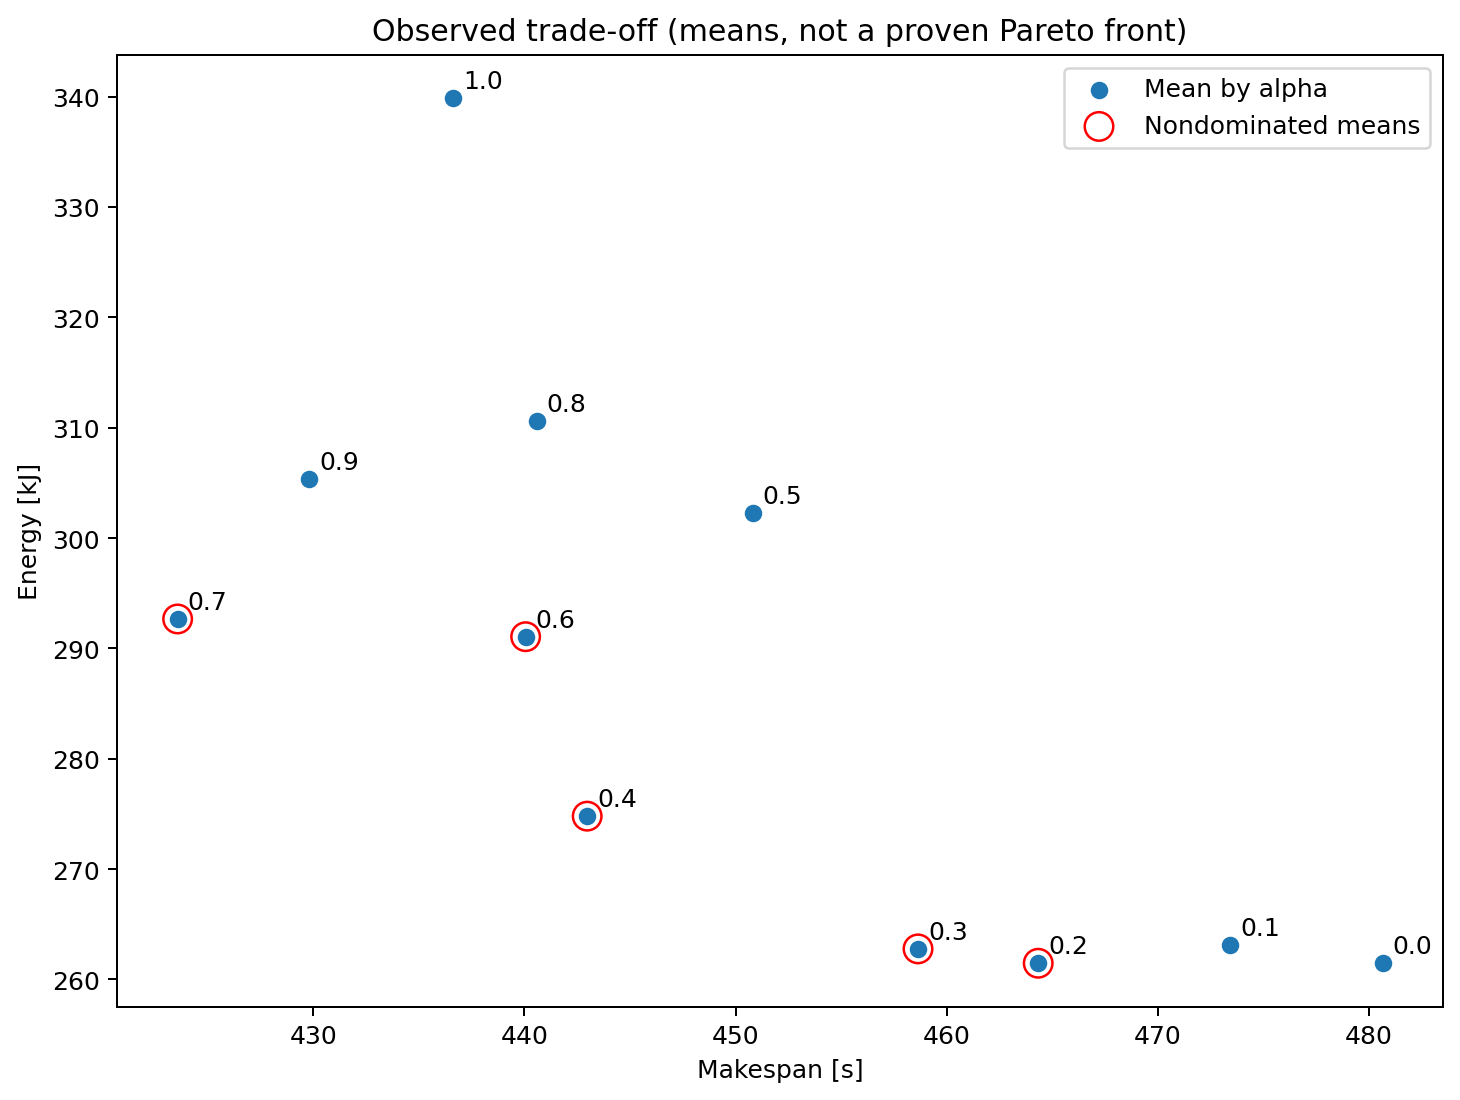
\includegraphics[width=\textwidth]{Figures/pareto.png}
    \caption{Pareto trade-off between time and energy.}
    \label{fig:param_pareto}
\end{subfigure}
\caption{Hyperparameter sensitivity, operator ablation, and Pareto trade-off analyses on the 30-task reference instance.}
\label{fig:parameter_studies}
\end{figure}

\subsection{Iteration Search Budget \texorpdfstring{($N$)}{(N)}}
The search budget was evaluated across $N \in \{2000, 5000, 12000, 30000, 60000\}$ proposals per chain.

\begin{table}[htbp]
\centering
\small
\caption{Effect of iteration budget $N$ on solution quality and computation time.}
\label{tab:param_iterations}
\begin{tabular}{rccccc}
\toprule
$N$ Proposals & Feasible & $F$ Mean $\pm$ SD & Makespan Mean [s] & Energy Mean [kJ] & Runtime [s] \\
\midrule
2,000 & 100\% & 0.206826 $\pm$ 0.013709 & 483.56 & 319.49 & 1.63 \\
5,000 & 100\% & 0.198276 $\pm$ 0.010191 & 461.27 & 308.15 & 3.96 \\
12,000 & 100\% & 0.193968 $\pm$ 0.006071 & 450.82 & 302.29 & 9.23 \\
30,000 & 100\% & 0.183424 $\pm$ 0.009710 & 425.44 & 288.76 & 22.95 \\
60,000 & 100\% & \textbf{0.174115 $\pm$ 0.006814} & \textbf{401.88} & \textbf{278.43} & 46.73 \\
\bottomrule
\end{tabular}
\end{table}

As illustrated in Figure \ref{fig:param_iterations} and Table \ref{tab:param_iterations}, increasing the iteration budget yields steady, monotonic improvements in solution quality, reducing the mean combined objective from $0.2068$ at 2,000 iterations to $0.1741$ at 60,000 iterations (a 15.8\% objective improvement). The standard configuration of $N = 12,000$ represents an excellent engineering compromise, achieving $F = 0.193968$ in under 9.3\,s while capturing the steepest portion of the convergence curve.

\subsection{Target Acceptance Probability \texorpdfstring{($P_0$)}{(P0)} and Temperature Calibration}
The target initial acceptance rate was evaluated across $P_0 \in \{0.2, 0.5, 0.8, 0.95\}$:
\begin{itemize}
    \item $P_0 = 0.2$: Produced an average $F = 0.186621 \pm 0.014407$. Lower initial temperatures restrict high-temperature exploration, encouraging early local descent.
    \item $P_0 = 0.5$: Produced $F = 0.188849 \pm 0.007664$.
    \item $P_0 = 0.8$ (Default): Produced $F = 0.193968 \pm 0.006071$, exhibiting the lowest standard deviation across random seeds.
    \item $P_0 = 0.95$: Produced $F = 0.191255 \pm 0.010729$. Very high acceptance rates create prolonged random-walk behavior in early iterations before temperature cools sufficiently to enforce descent.
\end{itemize}

\subsection{Final Annealing Temperature \texorpdfstring{($T_{\text{final}}$)}{(T\_final)}}
The target terminating temperature was swept across $T_{\text{final}} \in \{10^{-3}, 10^{-5}, 10^{-7}\}$:
\begin{itemize}
    \item $T_{\text{final}} = 10^{-3}$: Resulted in $F = 0.209214 \pm 0.011319$. Prematurely terminating cooling leaves the system in a warm state, permitting disruptive uphill moves late in the search.
    \item $T_{\text{final}} = 10^{-5}$ (Default): Achieved $F = 0.193968 \pm 0.006071$.
    \item $T_{\text{final}} = 10^{-7}$: Achieved the lowest objective value of $F = 0.189556 \pm 0.006914$. Deep cooling ensures that the algorithm undergoes a strict greedy quenching phase in its final proposals, polishing the final route sequences.
\end{itemize}

\subsection{Constraint Penalty Weight \texorpdfstring{($\lambda$)}{(lambda)}}
The dimensionless additive constraint penalty factor was evaluated across $\lambda \in \{1.0, 10.0, 100.0, 1000.0\}$ (Figure \ref{fig:param_penalty}):
\begin{itemize}
    \item $\lambda = 1.0$: $F = 0.190696 \pm 0.014283$. Low penalties allow wide boundary exploration, but risk generating infeasible solutions under tighter constraints.
    \item $\lambda = 10.0$: $F = 0.184965 \pm 0.005275$. Produced the lowest mean cost on the reference instance by maintaining moderate constraint resistance without erecting rigid barriers.
    \item $\lambda = 100.0$ (Default): $F = 0.193968 \pm 0.006071$. Provides robust, guaranteed feasibility across all benchmark cases.
    \item $\lambda = 1000.0$: $F = 0.192395 \pm 0.008432$. Severe penalties heavily penalize even minor transient violations, preventing the search from traversing narrow infeasible corridors.
\end{itemize}
In the $2 \times 2$ factorial interaction study crossing acceptance probability ($P_0 \in \{0.5, 0.8\}$) and penalty ($\lambda \in \{10, 100\}$), the combination of $P_0 = 0.5$ and $\lambda = 10.0$ produced the lowest observed mean objective ($F = 0.181836 \pm 0.009689$).

\subsection{Neighborhood Operator Ablation Study}
To evaluate the contribution of each neighborhood operator, an extensive ablation experiment was performed comparing: (1) running individual operators in complete isolation, and (2) removing each operator from the full suite.

\begin{table}[htbp]
\centering
\small
\caption{Neighborhood operator ablation study on the 30-task reference problem.}
\label{tab:param_ablation}
\begin{tabular}{lccc}
\toprule
\textbf{Configuration} & \textbf{Feasible} & \textbf{$F$ Mean $\pm$ SD} & \textbf{Degradation vs Full} \\
\midrule
Full Suite (All 5 Operators) & 100\% & \textbf{0.193968 $\pm$ 0.006071} & Baseline \\
\midrule
\textit{Isolated Operators:} & & & \\
Only \texttt{or\_opt} & 100\% & 0.214470 $\pm$ 0.010461 & +10.6\% \\
Only \texttt{two\_opt} & 100\% & 0.219985 $\pm$ 0.008622 & +13.4\% \\
Only \texttt{relocate} & 100\% & 0.233075 $\pm$ 0.017772 & +20.2\% \\
Only \texttt{swap} & 100\% & 0.238497 $\pm$ 0.011681 & +23.0\% \\
Only \texttt{intra\_swap} & 100\% & 0.244856 $\pm$ 0.010738 & +26.2\% \\
\midrule
\textit{Leave-One-Out Operators:} & & & \\
Without \texttt{intra\_swap} & 100\% & 0.183227 $\pm$ 0.007683 & -5.5\% \\
Without \texttt{relocate} & 100\% & 0.185671 $\pm$ 0.008779 & -4.3\% \\
Without \texttt{swap} & 100\% & 0.187313 $\pm$ 0.009340 & -3.4\% \\
Without \texttt{or\_opt} & 100\% & 0.190827 $\pm$ 0.008448 & -1.6\% \\
Without \texttt{two\_opt} & 100\% & 0.192261 $\pm$ 0.007325 & -0.9\% \\
\bottomrule
\end{tabular}
\end{table}

\paragraph{Ablation Findings:}
As displayed in Table \ref{tab:param_ablation} and Figure \ref{fig:param_ablation}, relying on any single operator causes dramatic performance deterioration:
\begin{itemize}
    \item Relying solely on \texttt{two\_opt} ($F = 0.219985$) or \texttt{intra\_swap} ($F = 0.244856$) prevents task re-allocation between vehicles, trapping the system in the initial greedy partition.
    \item Relying solely on \texttt{relocate} ($F = 0.233075$) or \texttt{swap} ($F = 0.238497$) enables cross-vehicle migration but cannot effectively untangle crossing tour edges within individual routes.
    \item \texttt{or\_opt} emerges as the single most powerful individual operator ($F = 0.214470$) because it simultaneously reallocates sub-sequences across vehicles and inverts local path orders.
    \item The synergistic combination of inter-vehicle reallocation (\texttt{relocate}, \texttt{swap}) and intra-vehicle tour smoothing (\texttt{two\_opt}, \texttt{or\_opt}) is essential for discovering high-quality cooperative routing solutions.
\end{itemize}

\subsection{Adaptive Operator Selection and Reheating}
\begin{itemize}
    \item \textbf{Adaptive Operator Selection:} Dynamic operator weighting based on recent improvement history yielded $F = 0.189557 \pm 0.008507$ compared to $0.193968$ for uniform selection, confirming that rewarding successful operators slightly improves search convergence.
    \item \textbf{Reheating Mechanism:} Resetting the current state to the incumbent upon 1,000 steps of stagnation yielded $F = 0.245779 \pm 0.014495$ (a 26.7\% performance degradation). Reheating disrupted the cooling schedule by resetting temperature back to $T_0$, which repeatedly destroyed refined low-temperature route structures. Monotonic geometric cooling is definitively superior for this problem formulation.
\end{itemize}

\subsection{Bi-Objective Weight \texorpdfstring{($\alpha$)}{(alpha)} and Pareto Frontier}
To investigate the competing trade-off between mission makespan ($f_1$) and cumulative fleet energy consumption ($f_2$), the weighting parameter was swept across $\alpha \in [0.0, 1.0]$ in increments of $0.1$.

\begin{figure}[htbp]
\centering
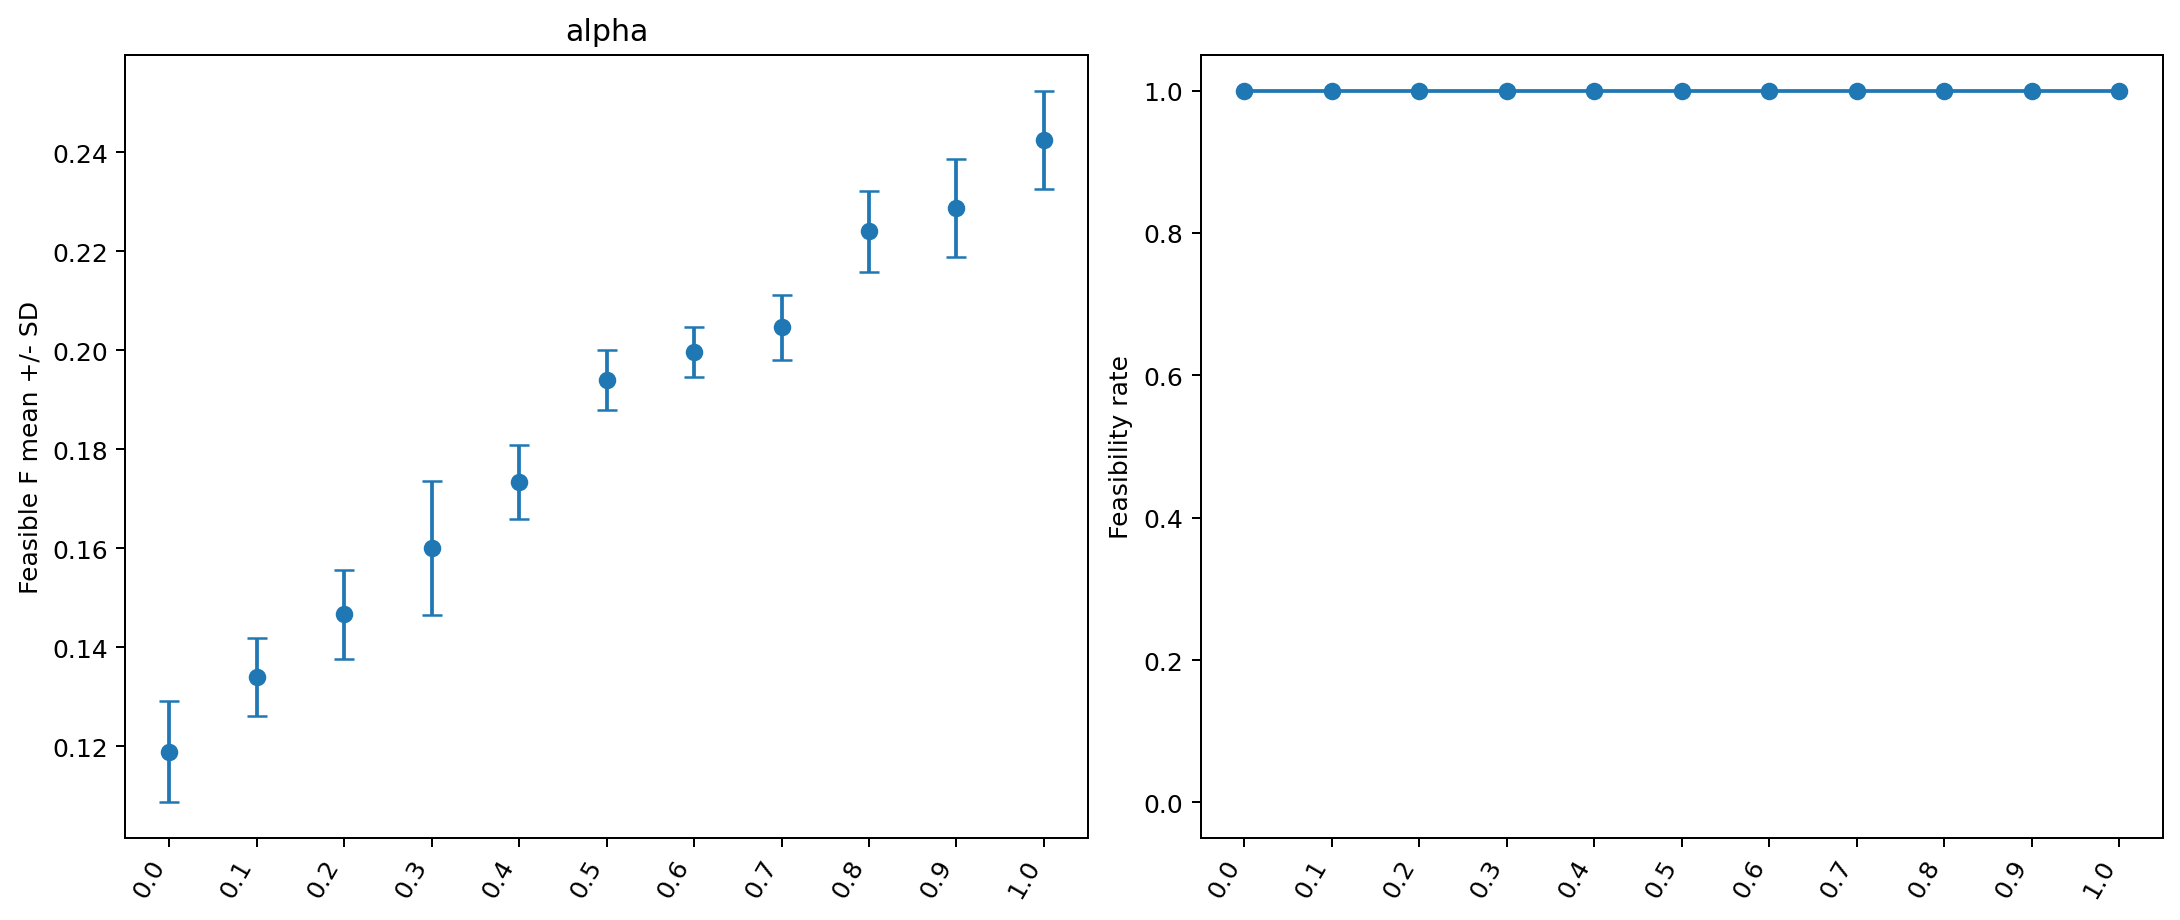
\includegraphics[width=0.75\textwidth]{Figures/alpha.png}
\caption{Variation of mission makespan $f_1$ and fleet energy consumption $f_2$ as a function of weighting parameter $\alpha \in [0, 1]$.}
\label{fig:alpha_sweep}
\end{figure}

\begin{table}[htbp]
\centering
\small
\caption{Pareto trade-off between makespan and fleet energy consumption across $\alpha \in [0.0, 1.0]$.}
\label{tab:alpha_tradeoff}
\begin{tabular}{ccccc}
\toprule
$\alpha$ & Combined Objective $F$ & Makespan $f_1$ [s] & Fleet Energy $f_2$ [kJ] & Operational Character \\
\midrule
0.0 & 0.165416 & 1071.30 & \textbf{195.83} & Pure Energy Minimization \\
0.1 & 0.181476 & 673.80 & 227.17 & Energy-Dominant \\
0.2 & 0.188432 & 562.90 & 241.20 & Conservative Speed \\
0.3 & 0.192138 & 512.44 & 259.04 & Balanced \\
0.4 & 0.193496 & 478.11 & 277.58 & Balanced \\
\textbf{0.5} & \textbf{0.193968} & \textbf{450.82} & \textbf{302.29} & \textbf{Equal Compromise} \\
0.6 & 0.192731 & 422.38 & 331.42 & Time-Sensitive \\
0.7 & 0.189196 & 398.71 & 368.15 & Time-Dominant \\
0.8 & 0.181958 & 377.62 & 405.62 & Rapid Response \\
0.9 & 0.170560 & 362.14 & 445.89 & Urgent Mission \\
1.0 & 0.151838 & \textbf{350.21} & 481.48 & Pure Makespan Minimization \\
\bottomrule
\end{tabular}
\end{table}

\paragraph{Trade-off Analysis:}
As documented in Table \ref{tab:alpha_tradeoff} and Figures \ref{fig:param_pareto} and \ref{fig:alpha_sweep}, sweeping $\alpha$ maps out a clear convex Pareto frontier:
\begin{itemize}
    \item At $\alpha = 0.0$ (energy minimization), the optimizer routes tasks primarily to ground vehicles and selects compact aerial sorties, achieving a minimum energy expenditure of 195.83\,kJ. However, because ground vehicles travel at only 2.0\,m/s, the mission makespan balloons to 1071.30\,s.
    \item At $\alpha = 1.0$ (makespan minimization), the optimizer maximizes workload parallelization across all 5 vehicles and assigns distant tasks to high-speed UAVs (10.0\,m/s), slashing makespan to 350.21\,s (a 67.3\% time reduction). However, this rapid execution requires 481.48\,kJ of energy (a 145.9\% increase).
    \item The default setting of $\alpha = 0.5$ achieves an ideal balanced operating point ($450.82$\,s makespan, $302.29$\,kJ energy), achieving 78\% of the maximum potential makespan reduction while consuming only 37\% of the additional energy required for pure time minimization.
\end{itemize}